\documentclass[12pt,a4paper]{article}
\usepackage[utf8]{inputenc}
\usepackage[czech]{babel}
\usepackage[T1]{fontenc}
\usepackage{amsmath}
\usepackage{amsfonts}
\usepackage{amssymb}
\usepackage{graphicx}
\usepackage[left=3cm,right=3cm,top=3cm,bottom=3cm]{geometry}
\usepackage{enumitem}

\begin{document}

\begin{center}
    \textbf{\Large Průběžná olympiáda z fyziky mladších}
    \vspace{1em}
    
    \textbf{Odevzdání do 22:59:59 SEČ, 3. 8. 2023 gregoriánského kalendáře}
\end{center}
\vspace{1em}

\begin{enumerate}[label=\arabic*)]

\item (3 body) Mějme vektory
\begin{equation*}
    \vec{u} = \left(4,\, 3.5,\, \frac{2}{3}\right),\quad \vec{v} = \left(0,\, 3,\, -4\right) ~.
\end{equation*}
Spočtěte $\vec{w} = \vec{u}\times\vec{v}$ a pomocí skalárního součinu určete úhly, které mezi sebou jednotlivé vektory $\vec{u}$, $\vec{v}$ a $\vec{w}$ svírají.

\item (4 bodů)
Mějme vektory $\vec{a}$, $\vec{b}$ a $\vec{c}$. Vyjádřete dvojitý vektorový součin $\vec{a}\times\left(\vec{b}\times\vec{c}\right)$ pomocí skalárních součinů. Hint: rozepište si celý výraz do složek :-)

\item (3 body)
Víťa si zlomil nohu v bérci. Z jeho kolena do zlomeniny vede vektor $\vec{a} = \left(1,\, -1,\, -5\right)$ a ze zlomeniny ke kotníku $\vec{u} = \left(-1,\, 1,\, -1\right)$. Pomocí vektorů $\vec{a},\vec{u}$ spočtěte, o jaký úhel je třeba narovnat jeho nohu, aby zase mohl chodit, než si zlomí druhou.

%\item ()
%Mějme vektor $\vec{u} = \left(1,\, 1,\, -1\right)$. Určete vektor $\vec{v}$ v rovině $xy$, aby vektor $\vec{u}\times\vec{v}$ mířil svisle (podél osy $z$) a svou délkou akorát dosáhl na Měsíc.

\item (4 body) Spočtěte:
\begin{align*}
    &\frac{\mathrm{d}^n}{\mathrm{d}x^n}x^n,\quad n\in\mathbb{N} ~,\\
    &\frac{\mathrm{d}}{\mathrm{d}x}\left[\frac{1}{\mathrm{ln}\left(x\right)}\right] ~,\\
    &\frac{\mathrm{d}}{\mathrm{d}x} e^{\cos\left(x^{\sin\left(\pi\right)}\right)}     ~,\\
    &\frac{\mathrm{d}}{\mathrm{d}x}\left[x^3\sin\left(x\right)\right] ~.
\end{align*}

\end{enumerate}

\newpage
\begin{center}
    \textbf{\Large Průběžná olympiáda z fyziky mladších}
    \vspace{1em}
    
    \textbf{Odevzdání do 22:59:59, 9. 8. 2023 gregoriánského kalendáře}
\end{center}

\begin{enumerate}[resume,label=\arabic*)]

\item (2 body)
Napište básničku s fyzikální tématikou a předneste ji přede všemi u večeře.

\item (5 bodů)
V 15:30 (tento čas můžeme označit $t = 0$) vyrazil mravenec ze středu hodin po vteřinové ručičce o délce $l = 20\,\mathrm{cm}$ konstantní rychlostí (vzhledem k ručičce). Na její konec došel v 15:40. Zaveďte si souřadnou soustavu, v níž jsou hodiny v klidu, a vzhledem k ní zapište polohu mravence jako funkci času. Dále spočtěte rychlost a zrychlení mravence a rozložte zrychlení na tečné a normálové.

\item (5 body)
Na závěsu o délce $2.5\,\mathrm{m}$ visí dřevený kvádřík o hmotnosti $750\,\mathrm{g}$. Víťa do něj střílí pistolí kulku o hmotnosti $8\,\mathrm{g}$, načež se kulka v kyvadle zasekne a rozhoupe jej s maximální výchylkou o $42^\circ$. Jaká je rychlost kulky při vstupu do kyvadla?

\item (4 body)
Piráta silnic, Tomáše, nelze snadno přehlédnout na dálnici. Začíná tím, že prudce zrychluje a během několika sekund dosáhne rychlosti $150\,\mathrm{km}\cdot\mathrm{h}^{-1}$, což je mnohem více než povolený limit. Poté, co si všimne policejního auta v dálce, prudce sníží rychlost na $80\,\mathrm{km}\cdot\mathrm{h}$, aby se vyhnul pokutě. Avšak jakmile je policejní auto mimo dohled, Tomáš opět zrychlí na $140\,\mathrm{km}\cdot\mathrm{h}^{-1}$. Když se blíží k výjezdu z dálnice, prudce brzdí a zastaví těsně před výjezdem. Jeho rychlost je zakreslena v grafu níže jako funkce času. Zakreslete do grafu také jeho zrychlení jako funkci času a určete, jakou ujel celkovou vzdálenost.
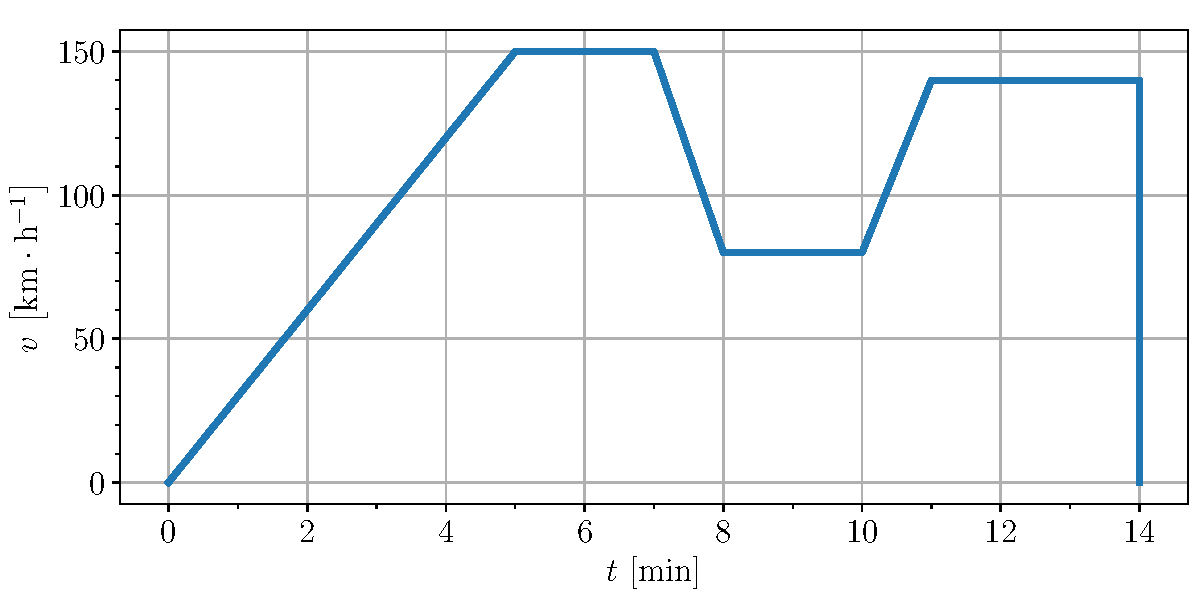
\includegraphics[width=0.9\textwidth]{tomas.pdf}

\item (4 body)
Had se pohybuje ze státní hranice v bodě $\left[-1\,\mathrm{m},\, 0\,\mathrm{m}\right]$ rovnoměrně přímočaře rychlostí $\left(3\,\mathrm{m}\cdot\mathrm{s}^{-1},\, 2\,\mathrm{m}\cdot\mathrm{s}^{-1}\right)$. Protože není proclený, celník za ním vyrazil ze strážní budky v bodě $\left[-1\,\mathrm{m},\, 2\,\mathrm{m}\right]$ rychlostí $\left(4\,\mathrm{m}\cdot\mathrm{s}^{-1},\, -1\,\mathrm{m}\cdot\mathrm{s}^{-1}\right)$, také rovnoměrně přímočaře. Najděte průsečík jejich trajektorií a rozhodněte, zda se v něm setkají. Určete čas, kdy si budou nejblíže, a jejich vzdálenost v tomto čase. Klikatění pohybu hada i celníka je zanedbatelné.

\item (3 body) Antiproton a pozitron v atomu antivodíku se navzájem přitahují jak Coulombovou, tak gravitační silou. Jaký je podíl velikostí těchto sil mezi nimi? Jako jejich vzdálenost uvažujte Bohrův poloměr $a_0 \doteq 0.529\cdot 10^{-10}\,\mathrm{m}$. Jak se odpověď změní při jiných hodnotách vzdálenosti?

\item (4 body) Bodová Helča o hmotnosti $m_H$ sedí na houpačce s pevným závěsem o délce 3 metry a Tomáš ji houpe. Musí ovšem náhle odběhnout, protože Víťa si zlomil nohu v Libérci, a Helču naposledy aspoň šťouchne o trochu víc, aby se vydržela déle houpat. To ji vytočí o půl otáčky, zastaví se přímo nad osou houpačky a spadne dolů. Jak rychle se pohybovala v nejnižším bodě houpačky?

\item (3 body) Spočtěte následující integrály:
\begin{align*}
    &\int 10^x \,\mathrm{d}x ~,\\
    &\int \frac{\sqrt{5\pi + \ln x}}{x} \,\mathrm{d}x ~,\\
    &\int_{-13}^{13} x^4\sin\left(x\right)\mathrm{d}x ~.
\end{align*}

\end{enumerate}

\end{document}
